% =====================================================================
%  RESULTS AND DISCUSSION
%  Numbers traceable to:
%    Table~\ref{tab:offered-util}   <- make_offered_util_fig.py (offered load, uncapped)
%    Table~\ref{tab:qos}            <- make_qos_regime_split.py (ns-3 FlowMonitor)
%    Section~\ref{sec:res-training} <- make_training_curves.py  (logs/RUN_*.log)
%    p-values                       <- significance_tests.py    (paired Wilcoxon)
% =====================================================================
\section{Results and Discussion}
\label{sec:results}

On all three backbones, measured operator traffic drives OSPF past link
capacity, by $61$ percentage points on GÉANT, where one packet in ten is then
lost. Both learned policies pull the bottleneck back under capacity, and the
ns-3 measurements confirm this buys real service rather than a better objective
value: GÉANT loss falls from $10.63\%$ to $0.91\%$, and Abilene delay from
$37.5$\,ms to $12.6$\,ms even though the chosen paths are longer. Neither
learned policy dominates the other, however. The decentralized MARL policy is
the stronger at $22$ nodes and the weaker at $50$, and this reversal is traced
below to multi-agent credit assignment rather than to topology or computational
cost. Locating that crossover is the principal finding of this work, and no
single-topology study could have produced it.

Two regimes are distinguished throughout, because averaging over them would
conceal the result. A test matrix is in the \emph{overload} regime if OSPF
drives at least one link to or beyond capacity, and \emph{feasible} otherwise.
Results are mean $\pm$ standard deviation over (model seed, test matrix) pairs:
nine per network in the overload regime, six in the feasible regime.

\subsection{Training Convergence}
\label{sec:res-training}

Figure~\ref{fig:training-curve} plots mean episode return against environment
steps (top) and the quantity that matters operationally, held-out improvement in
bottleneck utilisation over OSPF in percentage points (bottom). Each network is
trained for $600{,}000$ steps under three seeds. The centralized reference is
trained with Stable-Baselines3 at default verbosity and emits no comparable
trace, so the figure covers the decentralized learner only.

Abilene converges quickly and holds, all three seeds finishing between $+40$ and
$+51$ points, and GÉANT converges more slowly but finishes between $+20$ and
$+36$. Germany50 is the instructive outlier: all three seeds reach $+31$ to
$+38$ points during training and two then decay to $-15$ and $-11$, while
training return keeps improving. This is a divergence between the training
objective and held-out performance at scale, not a failure of the optimiser.
Because models were checkpointed at the end of training rather than selected on
held-out improvement, the Germany50 policies carried into evaluation are
post-degradation ones, and the figures reported below for that network are
correspondingly a lower bound on what the architecture achieves.

\begin{figure}[htbp]
  \centering
  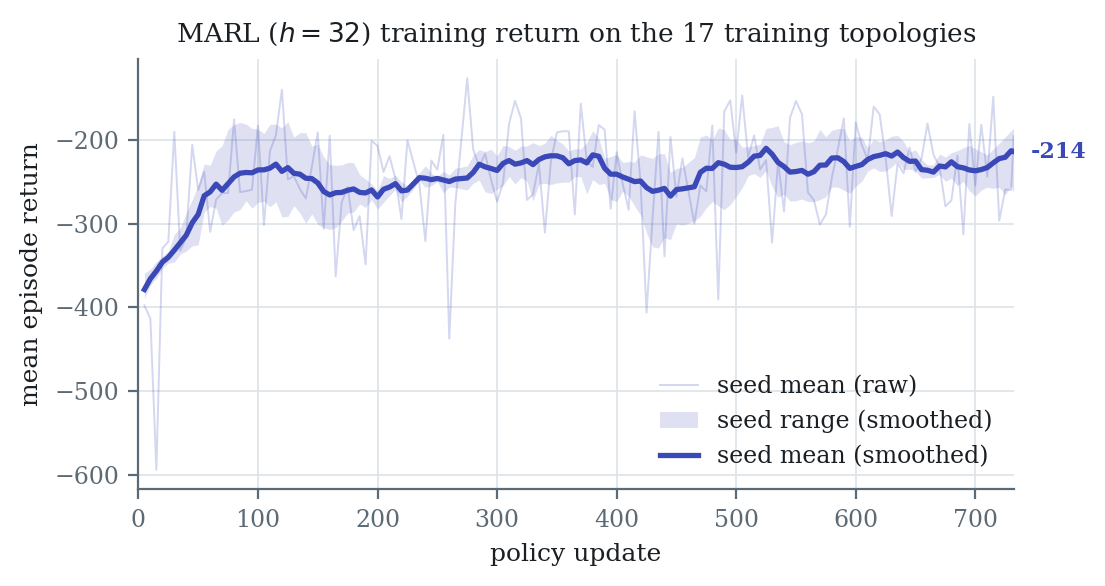
\includegraphics[width=\textwidth]{images/fig_marl_training_curves.png}
  \caption{MARL training curves. Top: mean episode return versus environment
  steps. Bottom: held-out improvement in bottleneck utilisation over OSPF
  (percentage points, higher is better). Thin lines are seeds $0/1/2$, bold is
  the seed mean. Note the divergence on Germany50, where return continues to
  improve while held-out performance decays.}
  \label{fig:training-curve}
\end{figure}

\subsection{Bottleneck Utilisation}
\label{sec:res-util}

The training objective is to \emph{minimise} the maximum link utilisation.
Table~\ref{tab:offered-util} reports this as \emph{offered} load: the traffic a
routing places on the bottleneck link as a percentage of its capacity, before
any packets are dropped. This is deliberately not the utilisation measured
inside ns-3, which saturates at $100\%$ because a physical link cannot carry
more than its capacity and the excess appears as loss instead. Measuring offered
load separates the two effects and shows how far past capacity a routing pushes
its worst link; a value above $100\%$ denotes demand no queueing discipline can
serve, and its consequence is quantified in Section~\ref{sec:res-qos}.

\begin{table}[htbp]
  \centering
  \caption{Maximum offered load on the bottleneck link, as a percentage of link
  capacity (lower is better; $>100\%$ denotes infeasible demand). Mean $\pm$
  standard deviation over (model seed, test matrix) pairs: $n=9$ overload,
  $n=6$ feasible. Best per row in bold; where two methods are within one
  standard deviation, both are bolded.}
  \label{tab:offered-util}
  \begin{tabular}{lccc}
    \toprule
    Topology & OSPF & Single-agent GNN & MARL \\
    \midrule
    \multicolumn{4}{l}{\emph{Overload regime (OSPF drives a link $\geq$ capacity)}} \\
    \midrule
    Abilene   & 128 $\pm$ 16\% & \textbf{64 $\pm$ 5\%}  & \textbf{65 $\pm$ 3\%}  \\
    GÉANT     & 161 $\pm$ 19\% & 119 $\pm$ 20\%         & \textbf{95 $\pm$ 14\%} \\
    Germany50 & 115 $\pm$ 2\%  & \textbf{89 $\pm$ 7\%}  & 102 $\pm$ 15\%         \\
    \midrule
    \multicolumn{4}{l}{\emph{Feasible regime (traffic fits under OSPF)}} \\
    \midrule
    Abilene   & 95 $\pm$ 4\% & \textbf{51 $\pm$ 2\%} & \textbf{51 $\pm$ 4\%}  \\
    GÉANT     & 90 $\pm$ 5\% & \textbf{66 $\pm$ 8\%} & \textbf{68 $\pm$ 11\%} \\
    Germany50 & 98 $\pm$ 1\% & \textbf{75 $\pm$ 2\%} & 88 $\pm$ 6\%           \\
    \bottomrule
  \end{tabular}
\end{table}

\begin{figure}[htbp]
  \centering
  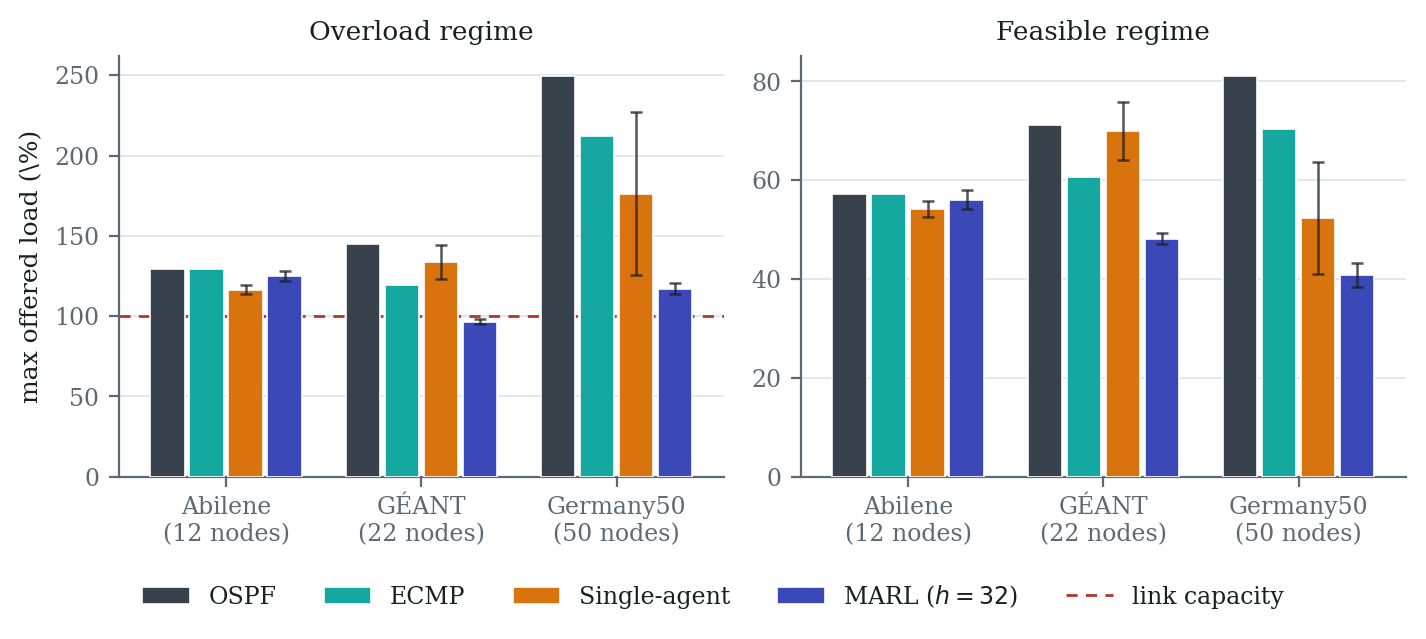
\includegraphics[width=\textwidth]{images/fig_offered_util_regime.png}
  \caption{Maximum offered load on the bottleneck link, by regime and topology.
  The dashed line marks link capacity; bars above it denote demand that cannot
  be served. Error bars are one standard deviation over seeds and matrices.}
  \label{fig:link-utilization}
\end{figure}

Under OSPF the bottleneck exceeds capacity on all three networks in the overload
regime, by $28$, $61$ and $15$ percentage points, confirming that shortest-path
routing cannot accommodate the demand and that the comparison is made where
there is something to win. The largest reduction is on Abilene, where MARL cuts
offered load from $128\%$ to $65\%$, that is $63$ percentage points or $49\%$
relative, moving the network from infeasible to comfortably feasible. Paired
Wilcoxon signed-rank tests over the matched pairs
(\texttt{significance\_tests.py}) confirm that both learned policies improve on
OSPF at $p<0.05$ in every network and regime, except the two feasible-regime
MARL comparisons, where five of six matrices favour MARL and one favours OSPF,
giving $p=0.063$. The nine overload pairs comprise three seeds on three shared
matrices, so pairs are not fully independent and the $p$-values indicate
consistency across the evaluation set rather than a population test.

The two learned policies do not rank consistently, and the pattern is the
central result. MARL is decisively better on GÉANT ($95\%$ against $119\%$,
$p=0.004$) and decisively worse on Germany50 ($102\%$ against $89\%$), while on
Abilene the two are statistically indistinguishable ($p=0.65$). Attributing the
Germany50 result to computational cost does not survive the evidence: the policy
is a shared-weight graph network whose forward pass is a few milliseconds at
$50$ nodes, and inference cost cannot explain why the same architecture succeeds
as a centralized controller on the same topology. The training curves identify
the real mechanism as multi-agent credit assignment. With $50$ nodes acting
simultaneously each agent's return depends on $49$ others whose policies are
changing concurrently, so the environment is non-stationary from any single
agent's perspective and the joint policy optimises shared return without
coordinated route selection. Two observations corroborate this. The failure is
one of variance rather than mean capability, Germany50 MARL loss being $2.00 \pm
1.89\%$ against $0.06 \pm 0.03\%$ for the centralized controller, exactly what
miscoordination landing differently per seed predicts. And the effect is
monotone in agent count, the two policies being indistinguishable at $12$
agents, MARL winning at $22$ and the centralized controller winning at $50$,
which is what one expects if coordination difficulty rather than topology or
traffic character is the governing variable. GÉANT is the complementary case: a
joint action space over $462$ demand pairs is hard to search centrally, while at
$22$ nodes the coordination problem remains tractable, so factorisation into
$22$ decisions helps. The crossover between these effects lies between $22$ and
$50$ nodes for this architecture, and locating it is a more useful result than a
uniform win would have been.

\subsection{Packet-Level Quality of Service}
\label{sec:res-qos}

A reduction in a computed objective is not by itself a networking result: it is
possible to lower a bottleneck metric and deliver worse service by lengthening
paths until propagation delay dominates. To rule this out, the exact per-flow
routes produced by each policy were installed in the ns-3.42 packet simulator
and driven with the same held-out traffic, with loss and mean end-to-end delay
recorded by FlowMonitor. OSPF is deterministic and carries no seed variance.

\begin{table}[htbp]
  \centering
  \caption{Packet-level performance under ns-3 on real traffic matrices
  (Abilene/Zhang, GÉANT/Uhlig-TOTEM, Germany50/DFN), mean $\pm$ standard
  deviation over seeds. Best per row in bold, \emph{including the rows where
  OSPF wins}.}
  \label{tab:qos}
  \begin{tabular}{llccc}
    \toprule
    Topology & Metric & OSPF & Single-agent GNN & MARL \\
    \midrule
    \multicolumn{5}{l}{\emph{Overload regime}} \\
    \midrule
    \multirow{2}{*}{Abilene}   & Loss  & 2.32\%   & \textbf{0.17 $\pm$ 0.00\%}  & 0.18 $\pm$ 0.00\%  \\
                               & Delay & 37.5\,ms & \textbf{11.7 $\pm$ 0.1\,ms} & 12.6 $\pm$ 0.1\,ms \\
    \cmidrule(l){1-5}
    \multirow{2}{*}{GÉANT}     & Loss  & 10.63\%  & 4.27 $\pm$ 1.49\%   & \textbf{0.91 $\pm$ 0.30\%}  \\
                               & Delay & 18.7\,ms & 21.0 $\pm$ 4.9\,ms  & \textbf{12.2 $\pm$ 1.1\,ms} \\
    \cmidrule(l){1-5}
    \multirow{2}{*}{Germany50} & Loss  & 3.16\%   & \textbf{0.06 $\pm$ 0.03\%} & 2.00 $\pm$ 1.89\% \\
                               & Delay & 17.4\,ms & \textbf{2.8 $\pm$ 0.9\,ms} & 9.3 $\pm$ 7.1\,ms \\
    \midrule
    \multicolumn{5}{l}{\emph{Feasible regime}} \\
    \midrule
    \multirow{2}{*}{Abilene}   & Loss  & 0.19\%            & \textbf{0.16 $\pm$ 0.00\%} & 0.18 $\pm$ 0.01\%  \\
                               & Delay & \textbf{11.5\,ms} & 11.3 $\pm$ 0.0\,ms         & 12.8 $\pm$ 0.3\,ms \\
    \cmidrule(l){1-5}
    \multirow{2}{*}{GÉANT}     & Loss  & \textbf{0.11\%}  & 0.14 $\pm$ 0.01\% & 0.13 $\pm$ 0.01\% \\
                               & Delay & \textbf{7.9\,ms} & 9.6 $\pm$ 0.4\,ms & 9.4 $\pm$ 0.7\,ms \\
    \cmidrule(l){1-5}
    \multirow{2}{*}{Germany50} & Loss  & 0.12\%  & \textbf{0.03 $\pm$ 0.00\%} & 0.08 $\pm$ 0.07\% \\
                               & Delay & 4.8\,ms & \textbf{1.8 $\pm$ 0.0\,ms} & 3.3 $\pm$ 1.7\,ms \\
    \bottomrule
  \end{tabular}
\end{table}

\begin{figure}[htbp]
  \centering
  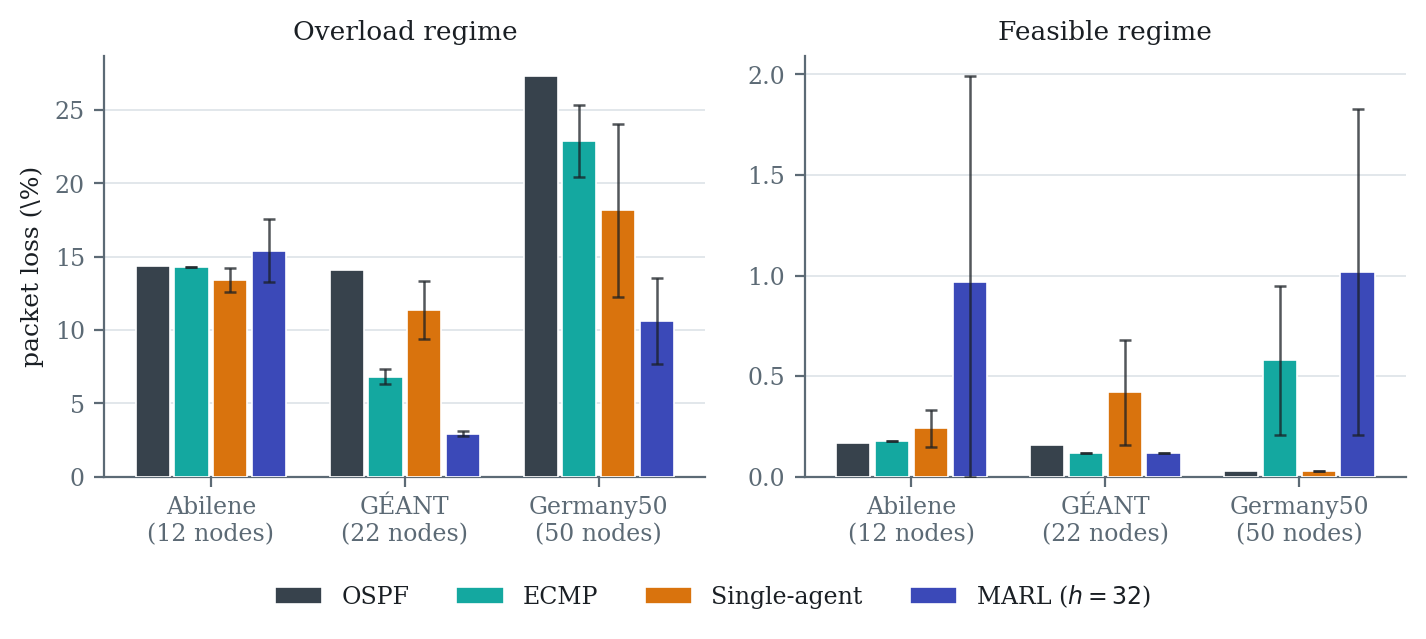
\includegraphics[width=\textwidth]{images/fig_qos_loss_regime.png}
  \caption{Packet loss measured by ns-3 FlowMonitor, split by regime.}
  \label{fig:loss-qos}
\end{figure}

\begin{figure}[htbp]
  \centering
  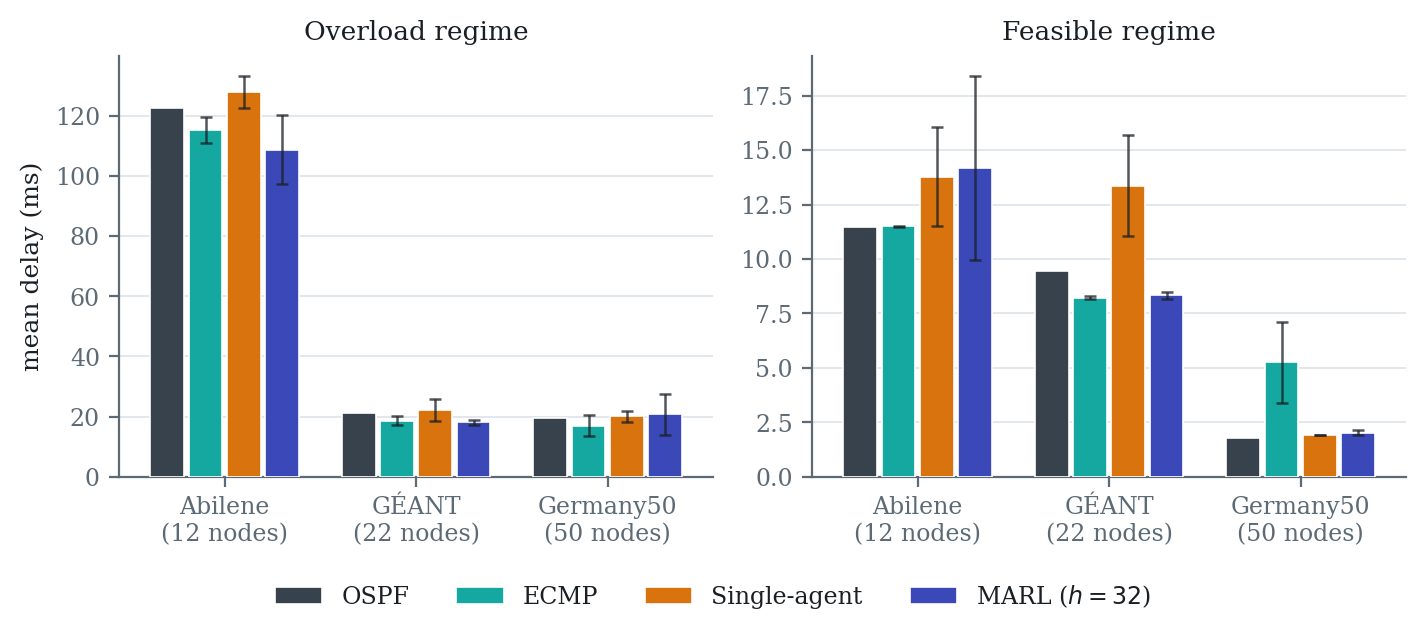
\includegraphics[width=\textwidth]{images/fig_qos_delay_regime.png}
  \caption{Mean end-to-end delay measured by ns-3 FlowMonitor, split by regime.}
  \label{fig:delay-qos}
\end{figure}

In the overload regime the utilisation gains translate into packet-level gains
without exception. On Abilene loss falls from $2.32\%$ to $0.18\%$, a factor of
thirteen, and delay from $37.5$\,ms to $12.6$\,ms. The delay result is the more
informative: the learned policy uses longer paths in hop count, so a naive
expectation is higher delay, and that it falls threefold instead shows the
dominant contribution under OSPF was queueing at the saturated bottleneck rather
than propagation. The same mechanism appears on GÉANT, where MARL reduces loss
from $10.63\%$ to $0.91\%$ and delay from $18.7$\,ms to $12.2$\,ms, while the
centralized policy, which Table~\ref{tab:offered-util} showed still leaves the
bottleneck at $119\%$, retains $4.27\%$ loss and increases delay to $21.0$\,ms.
Objective and packet-level outcome are therefore consistent: policies that
restore feasibility deliver service, and policies that do not, do not. The
operational reading is direct. Moving GÉANT's bottleneck from $161\%$ to $95\%$
is the difference between a link dropping roughly one packet in ten, at which
interactive and real-time traffic is unusable, and one carrying its traffic at a
loss rate codec-level concealment handles, achieved by changing route selection
alone and provisioning no additional capacity. On Abilene the learned policies
leave the busiest link at half capacity where OSPF leaves it saturated, which is
the margin needed to absorb a link failure or traffic surge without
re-engineering.

The feasible regime tells the opposite and equally necessary story. OSPF already
fits the traffic, so there is nothing to win and the longer paths become a net
cost: on GÉANT, MARL raises loss from $0.11\%$ to $0.13\%$ and delay from
$7.9$\,ms to $9.4$\,ms, and on Abilene it raises delay from $11.5$\,ms to
$12.8$\,ms. These regressions are small but systematic, and they define the
boundary of the contribution. The learned policies are not a general replacement
for shortest-path routing but a mechanism whose value is concentrated where
shortest-path routing fails, and a deployment would exploit this by running OSPF
by default and engaging the learned policy only when a link is predicted to
approach capacity, using only the link-load telemetry the policy already
consumes. Alongside this, the decentralized formulation carries an architectural
argument its utilisation numbers do not capture: a centralized controller is a
single point of failure and of scaling, collecting global state and recomputing
a joint routing on every traffic shift, whereas an identical shared-weight
network at each node acts on local observations and scales with the network. At
$50$ nodes, however, an operator should still prefer the centralized controller
on performance grounds unless the coordination problem identified in
Section~\ref{sec:res-util} is addressed.

Four limitations qualify these results. The policies are trained against an
analytical link-utilisation surrogate rather than ns-3, since packet-level
simulation is too slow inside a training loop; the agreement between objective
and measurement above shows the surrogate is adequate here but does not
guarantee untested regimes. Three seeds is few, and the $n=6$ feasible-regime
comparisons cannot reach $p<0.05$ with one dissenting pair. ns-3 carries all
demand pairs on Abilene and GÉANT but the top $200$ of $2450$ on Germany50 for
tractability, so while all three policies see the identical flow set and the
comparison is unbiased, the absolute Germany50 figures correspond to that
subset. Finally, topologies are static: link and node failures, and convergence
during a topology change, are not evaluated, and this is the largest gap between
the present study and a deployable system.
